\chapter{특수 상대성 이론: 기준계, 동시성, 로런츠 변환}

상대성 원리는 물리 법칙이 우리가 기술에 사용하는 관성계에 좌우되지 않는다는 원리다. 먼저 다룰 것은 운동학이다. 즉 공간, 시간, 운동, 동기화의 의미와 한 관성계에서 다른 관성계로의 변환을 살펴본다. 그다음에는 상대론적 에너지, 운동량, 힘, 뉴턴 운동 방정식에 해당하는 식, 그리고 \(E=mc^2\)의 의미를 포함한 동역학을 다룬다. 이 틀이 확립되면 아인슈타인 장 방정식을 푸는 어려운 문제부터 시작하지 않고도, 곡률 시공간, 주어진 중력장 속 입자의 운동, 블랙홀, 우주의 팽창을 통해 개념적으로 일반 상대성 이론에 접근할 수 있다.

개념적 엄밀성과 수학적 엄밀성을 구별할 필요가 있다. 우리는 틀린 줄 알면서 근사를 사용하지 않을 것이다. 대신 장 방정식의 임의의 해를 구성하는 데 필요한 수학적 도구는 뒤로 미루고, 중력장이 시계와 입자, 기하에 미치는 영향을 강조할 것이다. 이후의 모든 추론이 특수 상대성 이론의 운동학에 기반하므로, 특수 상대성 이론은 더 명시적으로 다루어야 한다.

따라서 출발점은 널리 알려진 공식이 아니라, 관찰자가 장소와 시간을 무엇으로 이해하는지에 관한 정확한 설명이어야 한다.

\section{기준계는 물리적 좌표계다}

공간에 아주 촘촘한 격자 모양으로 미터 자가 놓여 있다고 상상해 보자. 격자의 각 점에는 세 개의 공간 좌표가 부여되고, 각 점마다 시계가 하나씩 놓여 있다. 이 자와 시계를 합쳐 기준계라고 한다.

\begin{definition}
\emph{사건}이란 한 장소에서 한 시각에 일어나는 일이다. 공간이 한 차원일 때 좌표는 \((x,t)\)로 쓰고, 세 차원일 때는 \((x,y,z,t)\)로 쓴다.
\end{definition}

뉴턴 물리학은 강력한 가정을 하나 더한다. 모든 이상적인 시계는 한 번 동기화하면 계속 동기화된 상태를 유지할 수 있다는 가정이다. 시간은 보편적이다. 시계를 옮기거나 관찰자가 시계를 휴대할 수는 있지만, 모두가 어디서나 같은 \(t\)에 동의한다고 본다. 이를 절대 시간이라고도 한다. 온 세상을 위한 하나의 시계, 곧 신의 시간이라고 생각해도 좋다.

상대성 원리는 아인슈타인보다 오래된 개념이다. 완벽하게 매끄러운 선로 위를 기차가 아주 일정하게 달려서 흔들림이 전혀 없다고 상상해 보자. 기차 안에서는 역에 정차한 기차에서와 똑같이 공을 던지고 받을 수 있다. 공을 저글링하는 일은 놀랄 만큼 완결된 작은 역학 실험이다. 시간을 재고, 중력을 고려하고, 위치를 맞추며, 궤적을 반복해서 제어해야 하기 때문이다. 기차가 일정한 속도로 움직인다면 이런 규칙은 하나도 달라지지 않는다. 공을 수직으로 던지면 같은 손으로 돌아온다. 기차가 공 아래에서 미끄러져 나가지 않는다. 갈릴레이는 이 사실을 알아차렸고, 뉴턴은 운동 법칙으로 이를 체계화했다.

갈릴레이 이전에는 움직이는 기차가 공이 공중에 있는 동안 앞으로 나아가므로, 저글링하는 사람이 공을 받으려면 뒤나 앞으로 손을 뻗어야 한다고 생각하기 쉬웠다. 공이 손을 떠나는 순간 이미 기차의 수평 속도를 함께 지니고 있다는 점을 잊은 것이 오류다. 매끄럽게 움직이는 객차 안에서만 하는 실험으로는 특별한 절대 정지 상태를 알아낼 수 없다. 관측 가능한 것은 두 기차 사이의 상대 운동뿐이다.

따라서 정지한 기차와 일정한 속도로 움직이는 기차는 두 관성계다. 아인슈타인 이전에는 이 둘을 갈릴레이 변환으로 연결했다.

\section{시공간 그리기}

일단 \(y\)와 \(z\)는 생략하고, 시간은 세로축에, 위치 \(x\)는 가로축에 나타내자. 그림의 모든 점은 사건이다. 직선 \(x=0\)은 공간 원점의 이력, 즉 \emph{세계선}이다. 그에 이웃한 수직선 \(x=1,2,3,\ldots\)은 다른 격자점들의 세계선이다. 수평선은 시간이 같은 사건들의 집합이다.

\begin{figure}[H]
\centering
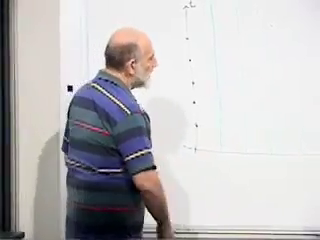
\includegraphics[width=0.62\textwidth]{lecture_01_figure_02.png}
\caption{정지계의 시간축과 공간 격자의 첫 세계선들.}
\lectureframe{00:16:38}
\end{figure}

같은 구성을 이상화한 그림으로 나타내면 더 분명하다.

\begin{figure}[H]
\centering
\begin{tikzpicture}[scale=0.95]
\draw[->] (-1.2,0) -- (5.2,0) node[right] {$x$};
\draw[->] (0,-0.2) -- (0,4.8) node[above] {$t$};
\foreach \x in {-1,1,2,3,4}
  \draw[gray!65] (\x,0) -- (\x,4.4);
\foreach \y in {1,2,3,4}
  \draw[gray!65] (-1.0,\y) -- (4.4,\y);
\fill (0,0) circle (1.5pt);
\node[below left] at (0,0) {$0$};
\node[left] at (0,1) {$1$};
\node[left] at (0,2) {$2$};
\node[left] at (0,3) {$3$};
\node[below] at (1,0) {$1$};
\node[below] at (2,0) {$2$};
\node[below] at (3,0) {$3$};
\end{tikzpicture}
\caption{정지한 시공간 격자. 수직선은 위치가 일정한 점들을, 수평선은 시간이 일정한 점들을 나타낸다.}
\end{figure}

격자는 상상 속의 것이며 간격은 임의로 정할 수 있다. 미터, 센티미터, 마이크론을 쓰거나 물리적으로 의미 있는 더 작은 간격을 쓸 수도 있다. 격자의 목적은 모든 사건에 정확한 좌표를 부여하는 것이다.

이제 ‘기준계’라는 말은 실제적인 의미를 갖는다. 단순히 어떤 방향을 바라보는 관점이나 사람을 가리키는 말이 아니다. 기준계는 공간 전체에 펼쳐진 좌표 장치다. 사건이 주어지면 그곳의 자가 어디서 일어났는지 알려 주고, 그곳의 시계가 언제 일어났는지 알려 준다. 그러면 입자의 위치와 속도, 에너지, 물체의 온도, 나아가 운동량과 힘 같은 다른 물리량도 기준계 사이에서 비교할 수 있다. 가장 간단한 비교는 \(x\)와 \(t\)에 관한 것이므로, 여기서부터 시작하자.

이제 일정한 속도 \(v\)로 양의 \(x\) 방향을 따라 움직이는 기차에 두 번째 격자를 놓자. 두 원점은 \(t=0\)에 일치하도록 정한다. 그러면 움직이는 원점의 궤적은 다음과 같다.
\begin{equation}
x=vt.
\end{equation}
기차에 고정된 다른 모든 점은 기울어진 평행 세계선을 따라간다. 이 기울기는 시간이 지남에 따라 기차의 위치가 변한다는 기하학적 표현일 뿐이다.

기차의 뒤쪽 끝이 프라임 원점이라고 하자. \(t=0\)에는 역의 원점과 일치한다. 그보다 뒤의 시각 \(t\)에는 역 기준 좌표가 \(vt\)이다. 따라서 좌표 \(x\)에 있는 인접한 사건은 기차 원점에서 \(x-vt\)만큼 떨어져 있다. 이것이 변환식이 임의의 대수 규칙이 아니라 뺄셈 형태인 이유다.

역 기준계에서 사건의 좌표를 \((x,t)\), 기차 기준계에서 그 좌표를 \((x',t')\)라 하자. 갈릴레이와 뉴턴은 보편적 시간을 그대로 유지한다.
\begin{equation}
t'=t.
\end{equation}
시간 \(t\) 동안 움직이는 원점은 \(vt\)만큼 전진하므로, 그 원점에서 사건까지의 거리는 다음과 같다.
\begin{equation}
x'=x-vt.
\end{equation}
두 식을 합치면,
\begin{align}
t'&=t, & x'&=x-vt.
\label{eq:galilean-forward}
\end{align}
미분 표시가 없는 좌표를 구하면 역변환은 다음과 같다.
\begin{align}
t&=t', & x&=x'+vt'.
\label{eq:galilean-inverse}
\end{align}

\begin{figure}[H]
\centering
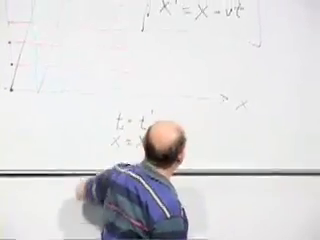
\includegraphics[width=0.72\textwidth]{lecture_01_figure_03.png}
\caption{두 시공간 격자 옆에 나타낸 갈릴레이 변환.}
\lectureframe{00:21:57}
\end{figure}

첫 번째 식은 움직이는 관찰자에게 정지한 관찰자가 준 좌표를 어떻게 변환할지 알려 준다. 역변환 쌍은 좌표를 다시 되돌린다. 두 기술 사이의 이 상호적인 변환이 갈릴레이 상대성의 수학적 내용이다.

역공간 변환식에서 \(t\to t'\)로 바꾸는 것은 갈릴레이 이론이 이미 \(t=t'\)라고 선언했기 때문에 문제가 없다. 이 가정을 지금 짚어 두는 것이 좋다. 아인슈타인 이론에서는 두 시간 좌표가 달라지므로, 이런 대입을 자동으로 할 수 없다.

\begin{classroomqa}
\audiencequestion{시계를 다른 곳으로 옮겼다가 다시 가져오면, 시계가 움직이는 동안 먼저 빨라졌다가 나중에 느려져 비교할 때 그 효과가 상쇄된 것은 아닌지 어떻게 알 수 있나요?
\lecturetimestamp{00:23:09}}
\lecturerresponse{갈릴레이는 오늘날의 정밀도로 보편적 시간을 확립할 수 없었다. 그것은 물리적 추측이었다. 좋은 시계를 서로 반대 방향으로 옮기거나, 동쪽--서쪽뿐 아니라 북쪽--남쪽으로도 이동을 반복하거나, 한 시계를 다른 시계 주위로 움직이거나, 시계를 한데 모으지 않은 채 시간 신호를 교환하는 등 여러 방법으로 이 추측을 시험할 수 있다. 일상적인 속도에서는 이런 시험이 모두 매우 높은 정밀도로 일치한다. 충분히 정밀한 시계나 충분히 큰 속도를 사용하면 작은 차이가 나타난다. 보편적 시간이 성립하지 않는다는 사실은 실험의 결함이 아니다. 이는 특수 상대성 이론이 설명해야 할 현상 중 하나다.}
\end{classroomqa}

\section{갈릴레이 불변량과 뉴턴 법칙}

불변량이란 논의 대상인 모든 관성계의 관찰자가 같은 값을 얻는 물리량이다. 좌표 자체가 불변일 필요는 없다. 중요한 것은 그 좌표로 세운 법칙이 같은 형태를 유지하는지 여부다.

이 말은 명사와 형용사로 모두 쓰인다. 수가 불변량일 수 있고, 방정식이 변환에 대해 불변일 수도 있다. 불변량과 불변 법칙을 구분하면 흔한 혼동을 피할 수 있다. 상대성 이론은 모든 관찰자가 모든 것에 대해 같은 좌표를 얻는다고 주장하지 않는다. 관측값 사이의 물리 법칙이 같은 형태를 갖는다고 주장한다.

위치 \(x_1\)와 \(x_2\)에 있는 두 사건이 동시에 일어난다고 하자. 식~\eqref{eq:galilean-forward}을 적용하면 다음과 같다.
\begin{align}
x_1'&=x_1-vt,\\
x_2'&=x_2-vt.
\end{align}
따라서 두 사건 사이의 거리는 다음과 같다.
\begin{equation}
x_2'-x_1'=(x_2-vt)-(x_1-vt)=x_2-x_1.
\end{equation}
갈릴레이 물리학에서는 같은 시각에 일어난 사건들 사이의 거리가 불변이다. 개별 위치는 불변이 아니더라도 그렇다.

\begin{classroomqa}
\audiencequestion{그 뺄셈에 나오는 \(t\)가 정말 같은 시각인가요?
\lecturetimestamp{00:28:16}}
\lecturerresponse{그렇다. 두 사건이 \((x_1,t)\)와 \((x_2,t)\)에 있도록 의도적으로 정했다. 두 사건은 하나의 수평 일정 시간선 위에 놓인다. 따라서 공통 항 \(vt\)은 소거된다. 사건들의 시각이 서로 달랐다면 이 논증으로 공간적 거리가 불변이라고 결론 내릴 수 없다.}
\end{classroomqa}

이제 입자의 궤적을 \(x(t)\)로 나타내자. 기차 안 관찰자는 다음과 같이 좌표를 정한다.
\begin{equation}
x'(t)=x(t)-vt.
\end{equation}
한 번 미분하면 익숙한 속도 합성 법칙이 나온다.
\begin{equation}
\frac{dx'}{dt}=\frac{dx}{dt}-v.
\end{equation}
위치와 속도는 기준계에 따라 달라진다. 화살을 나란히 따라 움직이는 관찰자는 선로 옆에 서 있는 관찰자보다 화살이 더 느리게 움직인다고 본다.

한 번 더 미분하자. 상대 속도 \(v\)는 일정하므로,
\begin{equation}
\frac{d^2x'}{dt^2}=\frac{d^2x}{dt^2}.
\end{equation}
가속도는 갈릴레이 변환 아래 불변이다. 뉴턴 법칙이 위치나 속도가 아니라 가속도로 쓰이는 이유가 여기에 있음을 알 수 있다.

여기서 말하는 것은 관찰 대상의 가속도이지, 기차 안 관찰자의 가속도가 아니다. 두 기준계는 관성계이므로 서로에 대해 가속하지 않는다. 어느 쪽 관점에서든 물체는 왼쪽이나 오른쪽으로 가속할 수 있다. 두 관찰자는 그 물체의 위치와 속도에는 동의하지 않지만 가속도 값에는 동의한다.

두 입자가 서로 힘을 미치고 그 힘이 두 입자 사이의 동시적 거리에만 의존한다고 하자. 그 거리는 불변이므로 힘도 불변이다. 질량 또한 물체에 고유하며 기준계와 무관한 성질이라면, 모든 관성계 관찰자는 다음을 쓸 수 있다.
\begin{equation}
F=ma
\end{equation}
그 형태는 완전히 동일하다. 뉴턴 역학은 갈릴레이 변환에 대해 불변이다. 이는 그럴듯한 주장에 그치지 않는다. 일상적인 속도의 영역에서 뉴턴 역학은 놀라울 정도로 정확하다.

이 논증은 거리의 함수로 크기가 정해지는 뉴턴 중력이나 정전기력 같은 익숙한 중심력에 적용된다. 모든 갈릴레이 관찰자는 같은 시각에 그 거리에 동의하므로 힘에도 동의한다. 힘과 가속도가 같다면 일관성을 위해 질량에도 동의해야 한다. 즉 기차가 지나가도 1킬로그램 물체는 여전히 1킬로그램이다. \(F=ma\)의 모든 기호는 같은 불변 구조를 따른다.

\section{빛에는 갈릴레이 법칙이 적용되지 않는다}

전자기학에서 문제가 생긴다. 맥스웰 방정식은 빈 공간을 일정한 속도 \(c\)로 이동하는 파동을 예측한다. 맥스웰 방정식이 자연 법칙이고 자연 법칙이 모든 관성계에서 동일하다면, 모든 관성계의 관찰자는 같은 \(c\)를 얻어야 한다.

갈릴레이 운동학은 다른 결과를 예측한다. 정지계에서 오른쪽으로 진행하는 빛 펄스는 다음을 만족한다.
\begin{equation}
x=ct.
\end{equation}
공간 변환을 적용하면,
\begin{equation}
x'=x-vt=(c-v)t.
\end{equation}
\(t'=t\)이므로 기차 안 관찰자는 속도를 \(c-v\)로 측정하게 된다.

모순은 명확하게 표현할 수 있다. 맥스웰 방정식의 형태가 유지된다면 프라임 기준계에서는 \(c\)를 예측한다. 갈릴레이 변환을 유지한다면 \(c-v\)를 예측한다. \(v\ne0\)일 때 두 결과가 모두 정확할 수는 없다.

빛이 매질 속에서 진행하는 보통의 파동처럼 행동한다고 보면 이 결과는 아주 자연스럽다. 물결과 함께 움직이는 배에서는 물결의 상대 속도가 더 낮게 측정된다. 정지한 공기 속을 움직이는 청자는 공기에 대한 자신의 운동에 따라 달라지는 음속을 측정한다. 따라서 19세기 물리학자들은 맥스웰 방정식이 가장 단순한 형태를 갖고 빛이 \(c\)로 움직이는, 우선적인 정지 상태인 에테르 기준계를 상정하게 되었다. 그러나 이 우선 기준계에 대한 운동을 검출하려고 설계한 실험에서는 그에 해당하는 효과가 발견되지 않았다.

가능한 실험 방법은 여럿이었지만, 모두 운동 상태나 방향이 서로 다른 관찰자들이 빛의 전파를 비교하는 것이 목적이었다. 어느 실험에서도 예상된 갈릴레이식 속도 이동은 나타나지 않았다. 이는 사소한 기술적 불편이 아니었다. 상대성 원리와 맥스웰 방정식, 그리고 물려받은 공간 및 시간 개념 중 무엇을 유지할지 선택해야 했다.

아인슈타인은 이 충돌을 더 직접적으로 다루었다. 젊은 시절 그는 빛의 파동을 뒤쫓는다고 상상했다. 빛을 따라잡을 수 있다면 진동하는 전자기파의 무늬가 공간에 정지한 것처럼 보일 테지만, 맥스웰 방정식은 그런 정지한 빛의 파동을 허용하지 않는다. 그는 맥스웰 이론과 상대성 원리를 근본 원리로 받아들이고, 좌표에 숨어 있는 가정을 다시 검토하기로 했다.

이 재구성은 두 가지 가정에 기초한다.
\begin{enumerate}
\item 물리 법칙은 모든 관성계에서 같은 형태를 갖는다.
\item 진공 속 빛의 속도 \(c\)는 모든 관성계에서 같다.
\end{enumerate}

두 번째 가정은 갈릴레이 변환과 양립할 수 없다. 속도 합성 법칙보다 더 근본적인 무언가가 바뀌어야 한다. 아인슈타인은 두 가정을 유지하고, 겉보기에는 무해한 갈릴레이 방정식 \(t'=t\)을 재검토하는 간결한 길을 택했다.

\section{멀리 떨어진 시계 동기화하기}

공간 거리는 자를 이용해 정할 수 있지만, 멀리 떨어진 시계에는 동기화 규약이 필요하다. 관찰자를 중심점에 두고 두 시계를 같은 거리만큼 떨어진 곳에 놓자. 양 끝 시계가 정해진 시각을 가리킬 때 각각 빛을 내보내게 한다. 두 빛이 중심점에 동시에 도착하면 양 끝 시계가 동기화되었다고 하자. 한쪽 빛이 먼저 도착하면 해당 시계를 조정하고 절차를 반복한다.

\emph{중점}이라는 말은 해당 기준계에 이미 놓인 자를 사용해 정의한다. 따라서 이 검정에는 서로 다른 두 요소가 들어 있다. 양 끝에서 같은 공간적 거리에 놓인 점이어야 하고, 신호의 도착 시각도 같아야 한다. 어느 한 요소도 생략할 수 없다. 격자 전체에서 이 절차를 반복하면 뉴턴이 그저 가정했던 수평 일정 시간선이 만들어진다.

이 정의에서 빛을 사용하는 이유는 가정에 따라 빛의 속도가 모든 관성계에서 같기 때문이다. 격자에서 이웃한 모든 시계 쌍에 이 절차를 적용하면 격자 전체에 동기화된 시계들이 배열된다.

이제 두 번째 격자가 첫 번째 격자 사이로 움직이게 하자. 움직이는 장치의 중점은 자체 기준계에서 움직이는 양 끝점의 한가운데에 계속 놓인다. 그러나 정지한 장치를 기준으로 보면 중점은 한쪽에서 다가오는 빛에 가까워지면서 다른 쪽 빛에서는 멀어진다. 정지한 시계 기준으로 동시에 방출된 빛은 움직이는 중점에 동시에 도착하지 않는다. 움직이는 관찰자도 같은 중점 및 빛 규칙을 적용하므로, 그 관찰자는 두 방출이 동시에 일어났다고 할 수 없다. 각 기준계는 자기 시계를 일관되게 동기화하지만, 두 동기화 결과는 서로 다르다.

이것은 빛의 유한한 이동 시간 때문에 생기는 착시가 아니다. 각 관찰자는 빛이 도착하는 데 시간이 걸린다는 점을 알고 있으며, 같은 속도 \(c\)를 사용해 이를 보정한다. 보정을 마친 뒤에도 두 관찰자가 동시 사건의 쌍으로 선택하는 멀리 떨어진 사건이 서로 다르므로 의견 차이가 남는다. 상대적인 것은 동시성의 겉모습만이 아니라 동시성 자체다.

\begin{classroomqa}
\audiencequestion{빛 대신 소리로 시계를 동기화하면 이 결론을 피할 수 있나요?
\lecturetimestamp{00:49:03}}
\lecturerresponse{공기가 정지한 기준계에서는 소리를 동기화 신호로 쓸 수 있지만, 측정되는 소리의 속도는 모든 관성계에서 같지 않다. 정지한 공기를 통과해 움직이는 개방된 기차는 소리를 전달하는 매질에 대해 움직이므로, 앞뒤 방향의 소리 신호는 대칭적으로 움직이지 않는다. 가정에 따르면 빛은 다르다. 어느 관찰자를 특별하게 만드는 검출 가능한 광학적 매질은 없다. 그러므로 우리는 빛을 사용하고 그 결과를 받아들인다.}
\end{classroomqa}

질적으로 어떤 의견 차이가 생기는지는 분명하다. 이제 움직이는 관찰자가 정확히 어떤 사건들을 동시라고 판단하는지 계산해 보자.

\section{빛 신호를 이용한 구성}

이 구성을 위해 다음과 같이 단위를 정하는 것이 편리하다.
\begin{equation}
c=1.
\end{equation}
그러면 거리 한 단위는 빛이 시간 한 단위 동안 이동하는 거리다. 예를 들어 초와 짝을 이루는 광초, 또는 년과 짝을 이루는 광년을 사용할 수 있다. 공간과 시간의 단위가 같아져 속도는 무차원이 되고, 빛은 그림에서 \(45^\circ\) 각도로 나타난다. 오른쪽으로 가는 빛은 다음을 만족한다.
\begin{equation}
x=t+d,
\end{equation}
왼쪽으로 가는 빛은 다음을 만족한다.
\begin{equation}
x=-t+d'.
\end{equation}
원점을 지나는 두 빛의 궤적은 각각 \(x=t\)와 \(x=-t\)이다. 빛보다 느린 물체의 시간꼴 궤적은 수직축에 더 가깝다. 가상의 초광속 궤적은 수평축에 더 가깝게 놓인다.

그림에서 각도는 이 단위를 선택한 뒤에야 의미가 있다. 미터와 초를 사용하면 빛은 일 초 동안 약 \(3\times10^8\)미터를 이동하므로 거의 수평으로 보일 것이다. 거리에 광초를 사용하면 가로축의 눈금이 조정되어 인과적 기하가 드러난다.

움직이는 격자에 있는 평행 세계선 세 개를 생각해 보자.
\begin{equation}
x=vt,\qquad x=vt+L,\qquad x=vt+2L.
\label{eq:moving-worldlines}
\end{equation}
가운데 세계선은 양 끝점 사이의 동시성을 검정하는 관찰자에 해당한다. 세 점 모두 등속 운동을 하며 프라임 기준계에서는 서로의 배치를 유지한다.

\begin{figure}[H]
\centering
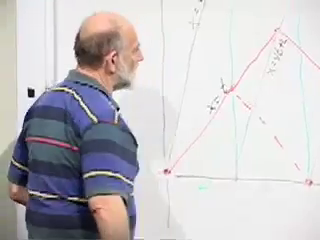
\includegraphics[width=0.72\textwidth]{lecture_01_figure_04.png}
\caption{가운데의 움직이는 세계선과 만나는 오른쪽 진행 빛 \(x=t\).}
\lectureframe{01:02:33}
\end{figure}

칠판 앞에 서 있는 사람이 가리지 않도록 전체 기하를 그려 보자.

\begin{figure}[H]
\centering
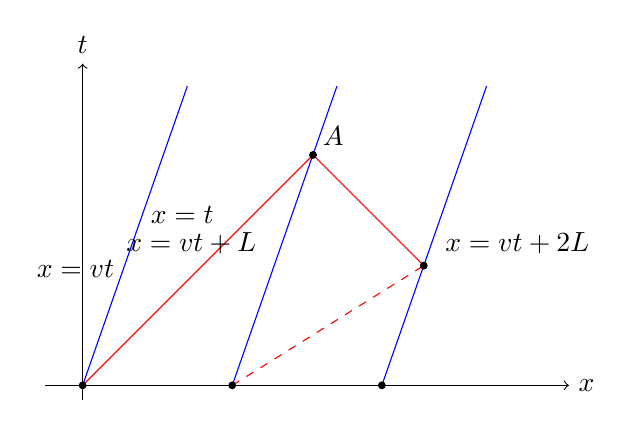
\begin{tikzpicture}[scale=0.95]
\draw[->] (-0.5,0) -- (6.5,0) node[right] {$x$};
\draw[->] (0,-0.2) -- (0,4.3) node[above] {$t$};
\draw[blue] (0,0) -- (1.4,4.0);
\draw[blue] (2.0,0) -- (3.4,4.0);
\draw[blue] (4.0,0) -- (5.4,4.0);
\draw[red] (0,0) -- (3.08,3.08);
\draw[red] (3.08,3.08) -- (4.56,1.60);
\draw[red,dashed] (2.0,0) -- (4.56,1.60);
\fill (0,0) circle (1.5pt);
\fill (2.0,0) circle (1.5pt);
\fill (4.0,0) circle (1.5pt);
\fill (3.08,3.08) circle (1.5pt);
\fill (4.56,1.60) circle (1.5pt);
\node[left] at (0.55,1.55) {$x=vt$};
\node[left] at (2.45,1.9) {$x=vt+L$};
\node[right] at (4.72,1.9) {$x=vt+2L$};
\node[left] at (1.88,2.28) {$x=t$};
\node[above right] at (3.08,3.08) {$A$};
\end{tikzpicture}
\caption{빛 신호가 움직이는 기준계의 동시성선을 정한다.}
\end{figure}

원점에서 오른쪽으로 가는 빛을 쏘자. \(A\)를 그 빛이 가운데 세계선과 만나는 사건이라고 하자. \(A\)에서 얻는 두 방정식은 다음과 같다.
\begin{align}
x&=t,\\
x&=vt+L.
\end{align}
대입하면 다음을 얻는다.
\begin{equation}
t=vt+L,
\end{equation}
따라서
\begin{equation}
t_A=x_A=\frac{L}{1-v}.
\label{eq:point-a}
\end{equation}

\(A\)에서 왼쪽으로 가는 빛을 따라 오른쪽 끝의 움직이는 세계선까지 거슬러 올라가자. 그 빛의 방정식은 다음 형태다.
\begin{equation}
x+t=b.
\end{equation}
이 빛은 \(A\)을 지나므로, 방정식~\eqref{eq:point-a}이 상수를 정해 준다.
\begin{equation}
b=x_A+t_A=\frac{2L}{1-v}.
\end{equation}
따라서 역방향 빛의 식은 다음과 같다.
\begin{equation}
x+t=\frac{2L}{1-v}.
\label{eq:backward-ray}
\end{equation}

오른쪽 끝 세계선과의 교점은 다음 두 식으로 구할 수 있다.
\begin{align}
x+t&=\frac{2L}{1-v},\\
x&=vt+2L.
\end{align}
\(x\)를 소거하면,
\begin{align}
(1+v)t
  &=2L\left(\frac{1}{1-v}-1\right)\\
  &=\frac{2Lv}{1-v},
\end{align}
따라서
\begin{equation}
t=\frac{2Lv}{1-v^2}.
\end{equation}
이를 \(x=vt+2L\)에 대입하면,
\begin{equation}
x=\frac{2L}{1-v^2}.
\end{equation}
좌표값 자체보다 두 좌표의 비가 중요하다.
\begin{equation}
\frac{t}{x}=v.
\end{equation}
그러므로 움직이는 시계 기준으로 원점과 동시에 일어나는 모든 사건은 다음 직선 위에 놓인다.
\begin{equation}
t=vx,
\label{eq:simultaneity-c-one}
\end{equation}
반면 움직이는 원점은 다음을 따른다.
\begin{equation}
x=vt.
\label{eq:moving-time-axis}
\end{equation}
두 축은 \(45^\circ\) 빛을 기준으로 대칭되게 기울어져 있다.

\(x=vt\) 위의 모든 점은 같은 프라임 위치 \(x'=0\)를 갖지만 프라임 시각은 달라진다. \(t=vx\) 위의 모든 점은 같은 프라임 시각 \(t'=0\)을 갖지만 프라임 위치는 달라진다. 따라서 한 직선은 프라임 시간축이고 다른 직선은 프라임 공간축이다. 두 번째 직선을 정하려면 긴 신호 구성이 필요했다. 움직이는 세계선만으로는 이를 추론할 수 없었다.

방정식~\eqref{eq:simultaneity-c-one}에 일반적인 단위를 복원하려면 다음이 필요하다.
\begin{equation}
t=\frac{v}{c^2}x.
\label{eq:simultaneity-dimensional}
\end{equation}
인자 \(c^2\)는 뉴턴적 그림이 일상생활에서 잘 들어맞는 이유를 설명한다. 속도가 \(c\)에 비해 아주 작으면 움직이는 동시성선의 기울기는 극히 작다.

\begin{figure}[H]
\centering
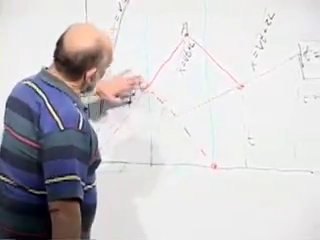
\includegraphics[width=0.72\textwidth]{lecture_01_figure_05.png}
\caption{\(c=1\)일 때 프라임 시간축과 동시성축은 빛을 기준으로 대칭이다.}
\lectureframe{01:15:40}
\end{figure}

\begin{figure}[H]
\centering
\begin{tikzpicture}[scale=1.0]
\draw[->] (-2.2,0) -- (5.2,0) node[right] {$x$};
\draw[->] (0,-0.2) -- (0,4.9) node[above] {$t$};
\draw[red] (0,0) -- (3.9,3.9);
\draw[red] (0,0) -- (-1.8,1.8);
\draw[blue] (0,0) -- (1.8,4.5);
\draw[blue,dashed] (0,0) -- (4.5,1.8);
\node[right] at (3.9,3.9) {$x=t$};
\node[left] at (-1.8,1.8) {$x=-t$};
\node[above] at (1.8,4.5) {$x'=0$};
\node[right] at (4.5,1.8) {$t'=0$};
\end{tikzpicture}
\caption{\(c=1\) 단위에서 프라임 축과 불변인 빛의 궤적.}
\end{figure}

\section{로런츠 변환 유도}

기하를 통해 각 프라임 좌표가 어디에서 영이 되는지 알 수 있다. 움직이는 시간축 \(x=vt\)에서는 \(x'=0\)이어야 한다. 움직이는 동시성축 \(t=vx\)에서는 \(t'=0\)이어야 한다. 이 영점 조건을 만족하는 가장 일반적인 선형 관계는 다음과 같이 쓸 수 있다.
\begin{align}
x'&=\frac{x-vt}{F(v)},\\
t'&=\frac{t-vx}{G(v)}.
\label{eq:fg-ansatz}
\end{align}
인자 \(F\)와 \(G\)는 축의 위치가 이미 정해졌더라도 프라임 좌표의 눈금이 갈릴레이식 눈금과 다를 수 있게 한다. 공간과 시간의 균질성으로부터 선형성이 따른다. 즉 실험을 평행 이동해도 변환 법칙은 달라지지 않는다.\editorialnote{이 짧은 선형성 논증은 칠판에서 유도할 때 암묵적으로 사용한 가정을 분명하게 드러낸다.}

이 단계에서 기하는 많은 것을 알려 주었지만 전부 알려 주지는 않았다. 분자는 축의 기울기를 정한다. 하지만 축을 따라 단위 간격이 어떻게 정해지는지는 알려 주지 않는다. 남은 눈금 정보가 바로 \(F(v)\)와 \(G(v)\)가 나타내는 것이다.

이제 빛의 속도가 불변이라는 조건을 부과하자. \(x=t\)를 따르는 오른쪽 진행 빛은 \(x'=t'\)도 만족해야 한다. 그 빛을 따라가면,
\begin{align}
x'&=\frac{(1-v)t}{F(v)},\\
t'&=\frac{(1-v)t}{G(v)}.
\end{align}
빛 궤적의 모든 점에서 이 관계가 성립하려면,
\begin{equation}
F(v)=G(v).
\end{equation}
따라서 다음과 같이 쓸 수 있다.
\begin{align}
x'&=\frac{x-vt}{F(v)},\\
t'&=\frac{t-vx}{F(v)}.
\label{eq:common-f}
\end{align}

이 단계에서는 대수적으로 처음으로 아인슈타인다운 요구 조건을 사용한다. 두 관찰자 모두에게 같은 기하학적 직선이 빛의 궤적이므로, \(c=1\)일 때 두 프라임 좌표는 그 선을 따라 똑같이 증가해야 한다. 두 식의 인자가 다르면 프라임 기준계에서 빛의 속도는 단위값과 달라진다.

미지 함수가 하나 남았다. 방정식~\eqref{eq:common-f}에 \(F(v)\)를 곱하면,
\begin{align}
F(v)x'&=x-vt,\\
F(v)t'&=t-vx.
\end{align}
두 번째 방정식에 \(v\)를 곱하고 첫 번째 식에 더하면 \(t\)가 소거되어 다음을 얻는다.
\begin{equation}
(1-v^2)x=F(v)(x'+vt').
\end{equation}
마찬가지로,
\begin{equation}
(1-v^2)t=F(v)(t'+vx').
\end{equation}
따라서 역변환은 다음과 같다.
\begin{align}
x&=\frac{F(v)}{1-v^2}(x'+vt'),\\
t&=\frac{F(v)}{1-v^2}(t'+vx').
\end{align}

상대성 원리에 따라 두 기준계는 서로 대칭적이다. 역에서는 기차가 \(+v\)로 움직이는 것으로 보인다면, 기차에서는 역이 \(-v\)로 움직이는 것으로 보인다. 따라서 역방정식은 \(v\)의 부호를 바꾼 같은 형태를 가져야 한다. 두 식의 앞 인자는 다음 조건을 만족해야 한다.
\begin{equation}
\frac{F(v)}{1-v^2}=\frac{1}{F(v)}.
\end{equation}
그러므로
\begin{equation}
F(v)^2=1-v^2,
\end{equation}
그리고 \(v=0\)에서 항등 변환과 연속이어야 하므로 양의 근을 택한다.
\begin{equation}
F(v)=\sqrt{1-v^2}.
\end{equation}

이 결과는 특정한 빛 펄스에 맞춰 조정한 것이 아니다. 동기화로 정해진 축, 빛의 공통 속도, 어느 관성계도 다른 관성계보다 우선하지 않는다는 요구에서 나온다.

\(c=1\)인 단위계에서 로런츠 변환은 다음과 같다.
\begin{align}
x'&=\frac{x-vt}{\sqrt{1-v^2}},\\
t'&=\frac{t-vx}{\sqrt{1-v^2}}.
\label{eq:lorentz-c-one}
\end{align}
역변환은 다음과 같다.
\begin{align}
x&=\frac{x'+vt'}{\sqrt{1-v^2}},\\
t&=\frac{t'+vx'}{\sqrt{1-v^2}}.
\end{align}

\begin{figure}[H]
\centering
\includegraphics[width=0.76\textwidth]{lecture_01_figure_06.png}
\caption{완성된 \(c=1\) 로런츠 변환을 칠판에 나타낸 모습.}
\lectureframe{01:32:38}
\end{figure}

핵심적인 새로움은 시간 방정식에 이미 드러나 있다. 시간은 한 기준계에서 다른 기준계로 그대로 옮겨지지 않는다. 프라임 시간 좌표에는 프라임이 없는 시간과 위치가 섞인다. 따라서 \(t=\text{constant}\)와 \(t'=\text{constant}\)는 서로 다른 사건 집합을 나타낸다.

이 혼합 항은 나중에 덧붙이는 선택적 보정 항이 아니다. 이 항이 없으면 \(t'=0\) 직선은 수평으로 남고, 멀리 떨어진 곳 사이의 동시성은 보편적인 채로 유지되며, 변환은 빛의 속도를 보존할 수 없다.

\section{빛의 속도 복원과 결과 검산}

\(c\ne1\)이면 차원 일관성을 위해 빠진 인자들을 복원해야 한다. 비 \(v^2/c^2\)는 무차원이고 \((v/c^2)x\)는 시간의 단위를 갖는다. 따라서
\begin{align}
x'&=\frac{x-vt}{\sqrt{1-v^2/c^2}},\\
t'&=\frac{t-(v/c^2)x}{\sqrt{1-v^2/c^2}}.
\label{eq:lorentz-dimensional}
\end{align}
\(v\)의 부호를 바꾸면 역변환을 얻는다.
\begin{align}
x&=\frac{x'+vt'}{\sqrt{1-v^2/c^2}},\\
t&=\frac{t'+(v/c^2)x'}{\sqrt{1-v^2/c^2}}.
\end{align}
다음을 도입하면,
\begin{equation}
\gamma=\frac{1}{\sqrt{1-v^2/c^2}}
\end{equation}
식은 익숙한 간결한 형태로 쓸 수 있지만, 분모 형태를 유지하면 유도 과정을 확인하기 쉽다.

수치로는 \(c\simeq3\times10^8\,\mathrm{m/s}\)이므로 \(c^2\simeq9\times10^{16}\,\mathrm{m^2/s^2}\)이다. 분모가 크기 때문에 대부분의 역학 실험에서는 동시성선의 기울기와 인자 \(v^2/c^2\)를 감지할 수 없다. 이 효과가 작은 덕분에 갈릴레이 역학이 성공했지만, 절대 시간이 되살아나는 것은 아니다.

\begin{figure}[H]
\centering
\includegraphics[width=0.76\textwidth]{lecture_01_figure_07.png}
\caption{인자 \(c\)를 복원한 로런츠 변환.}
\lectureframe{01:35:58}
\end{figure}

두 가지 점검을 바로 할 수 있다. 먼저 \(v\ll c\)로 두자. 그러면 \(v^2/c^2\)은 무시할 수 있고, 보통의 거리에서는 동시성의 상대성에 따른 항 \(vx/c^2\)도 무시할 수 있다. 식~\eqref{eq:lorentz-dimensional}은 다음과 같이 된다.
\begin{equation}
t'\approx t,\qquad x'\approx x-vt.
\end{equation}
저속 근사에서 갈릴레이 상대성이 회복된다.

둘째, 광선을 살펴보자. \(c\)를 다시 넣으면 오른쪽으로 진행하는 광선은 \(x=ct\)을 따르며, \(x=t\)을 따르지 않는다. 이를 대입하면 다음을 얻는다.
\begin{align}
x'&=\frac{(c-v)t}{\sqrt{1-v^2/c^2}},\\
t'&=\frac{(1-v/c)t}{\sqrt{1-v^2/c^2}}.
\end{align}
\(c-v=c(1-v/c)\)이므로,
\begin{equation}
x'=ct'.
\end{equation}
프라임 좌표계의 관측자도 같은 속력 \(c\)을 측정한다. 왼쪽으로 진행하는 광선에 \(x=-ct\)를 대입해도 마찬가지로 다음을 얻는다.
\begin{equation}
x'=-ct'.
\end{equation}
이 변환은 어느 방향으로 진행하는 빛에도 올바르게 적용된다.

\(x=t\)와 \(x=ct\)의 차이는 차원을 확인하는 데 유용하다. 전자는 \(c=1\)인 단위계에서만 옳다. 광선 방정식은 자연 단위계에 둔 채 변환식에만 보통 단위를 다시 넣으면 두 단위 관례가 뒤섞여 잘못된 결과가 나온다. 차원의 일관성을 확인하면 이 실수를 바로 알아낼 수 있다.

\section{중점 기준}

\begin{classroomqa}
\audiencequestion{관측자가 두 광원에서 나온 섬광을 동시에 받았지만 두 광원의 중간 지점에 있지는 않다고 하자. 이 관측자는 두 섬광이 동시에 방출되었다고 결론 내릴 수 있는가?
\lecturetimestamp{01:42:55}}
\lecturerresponse{아니다. 도착 시간이 같다는 사실로 방출 시간도 같다고 결론 내릴 수 있는 것은 관련 좌표계에서 두 광원의 공간적 중간에 있는 관측자뿐이다. 한 광원에 더 가까운 수신자는 더 먼 쪽의 섬광이 먼저 방출되었는데도 두 섬광을 동시에 받을 수 있다. 따라서 움직이는 구성에서는 중점 세계선 \(x=vt+L\)이 필수적이다. 정방향 광선 \(x=t\)을 그 중점에 닿을 때까지 따라간 뒤, 역방향 광선을 \(x=vt+2L\)까지 거슬러 추적한다. 그 두 번째 끝점 사건은 다른 곳에서 임의로 택한 도착 동시 사건이 아니라, 움직이는 좌표계에서 원점과 동시인 사건이다.}
\end{classroomqa}

좌표 변환 전체를 얻었지만, 이제 가장 익숙한 결과들을 살펴볼 차례다. 다음으로 길이 수축, 시간 지연, 고유 시간을 다루고, 이어서 상대론적 운동량과 에너지를 다룬다. 토대는 이미 마련되었다. 각 관성계가 같은 법칙을 쓰고 같은 빛의 속력을 측정할 수 있는 것은 공간과 시간이 서로 섞이고, 멀리 떨어진 사건의 동시성이 절대적으로 정해지는 것이 아니라 좌표계에 속하기 때문이다.
